\documentclass[10pt,twocolumn]{article}
\usepackage[margin=0.55in,top=0.58in,bottom=0.58in]{geometry}
\usepackage{amsmath,amssymb,amsthm}
\usepackage{booktabs}
\usepackage{graphicx}
\usepackage{microtype}
\usepackage[hidelinks]{hyperref}
\usepackage{xurl}

\raggedbottom
\setlength{\columnsep}{0.20in}
\setlength{\parskip}{1.4pt}
\setlength{\textfloatsep}{7pt plus 2pt minus 2pt}
\setlength{\dbltextfloatsep}{8pt plus 2pt minus 2pt}

\title{\vspace{-1.2em}\textbf{Exact Dual-Ring, Bini-Interpolation, and Constructive Lean~4 Certificates for Deterministic Real Matrix-Product Verification Complexity}\vspace{-0.4em}}
\author{Lluis Eriksson\\
\small Independent Researcher (\nolinkurl{https://github.com/lluiseriksson})\\
\small Companion Preprint to Chen Xiangle (\texttt{arXiv:2611.34814v1}) --- Unrefereed Formal-Verification Artifact\vspace{-0.6em}}
\date{November 26, 2026}

\begin{document}
\maketitle

\begin{abstract}
\noindent Chen Xiangle (\texttt{arXiv:2611.34814v1}, Nov.~2026) proves that any real arithmetic decision tree of cost $s$ deciding $y = T(u,v)$ for a bilinear map $T:\mathbb{R}^p\times\mathbb{R}^q \to \mathbb{R}^m$ implies $\underline{\mathrm{rank}}_{\mathbb{R}}(T) \le 30s$ (and $\underline{\mathrm{rank}}_{\mathbb{C}}(T_{\mathbb{C}}) \le 30s$), establishing that deterministic exact real matrix-product verification has the same arithmetic exponent $\omega_{\mathbb{C}}$ as matrix multiplication (giving a conditional $\Omega(n^{9/4}) = \Omega(N^{9/8})$ vs.\ $O(N)$ separation from Freivalds' randomized test under the Nov.~2026 OpenAI border-rank preprint) and matching $\Omega(S^{\omega_{\mathbb{C}}/2})$ white-box polynomial identity testing (PIT) lower and dense-quadratic upper bounds. We provide an independent, zero-floating-point companion certification suite (\texttt{DET-MATMUL-VERIF-CERT-1.0}) comprising: (i)~18 constructive theorems in Lean~4.35.0 (0~\texttt{sorry}, 0~custom axioms, 0~\texttt{Classical.choice}); (ii)~a zero-float Python verifier over exact $\mathbb{Q}$ and the dual ring $\mathbb{Q}[\alpha,\beta]/(\alpha^2,\beta^2)$ auditing Freivalds' soundness, the Baur--Strassen $30s$ rank chain, Bini's Laurent-truncation Lagrange interpolation, white-box PIT reductions, and the dense-quadratic Gram equivalence $RJR^T=0 \iff HJH=0$; and (iii)~16 canonical JSON certificates and 29 unit/forgery/AST tests. Our audit also documents and certifies the exact corrected aspect-ratio inequality $(b/a)a^\omega \le (ab)^{\omega/2}$ ($a\le b$) for Section~6's dense quadratic upper bound.
\end{abstract}

\section{Introduction and Scope}
Since Freivalds~\cite{Freivalds1979Fast} showed that randomized verification of $AB = C$ takes $O(n^2)$ arithmetic steps with one-sided error at most $1/2$ and B\"urgisser, Karpinski, and Lickteig~\cite{BurgisserKarpinskiLickteig1992} posed deterministic graph verification of real matrix multiplication, determining whether deterministic exact verification can beat the matrix multiplication exponent $\omega_{\mathbb{C}}$ remained open~\cite{Kunnemann2018Freivalds}. In~\cite{Chen2026DetVerif}, Chen Xiangle resolves this question in the real algebraic decision-tree model: by summing squares of vanishing path tests into $P = \sum_j z_j^2$, perturbing $P - w\cdot y$ so Sard's theorem yields invertible Jacobian $J = \partial_y F$, controlling mixed derivatives via semialgebraic quantifier elimination (Lemma~3), and tracking cross terms through a Baur--Strassen reverse-mode circuit~\cite{BaurStrassen1983} in the dual ring $\mathbb{R}[\alpha,\beta]/(\alpha^2,\beta^2)$, Chen proves $\underline{\mathrm{rank}}(T) \le 30s$ (Theorem~1), deducing $s = \Omega(n^{\omega_{\mathbb{C}}})$ via Bini's border-rank lemma~\cite{Bini1980BorderRank} (Corollary~2) and a conditional $\Omega(N^{1/8})$ gap over Freivalds under~\cite{OpenAI2026NineFourths}.

\paragraph{Scope and attribution.}
This note is an \emph{unrefereed companion verification preprint} to~\cite{Chen2026DetVerif}. All primary mathematical theorems and proof architecture belong exclusively to Chen Xiangle~\cite{Chen2026DetVerif}. Real-analytic/semialgebraic pillars (Hardt's $C^2$ decomposition, Tarski--Seidenberg quantifier elimination, Sard's theorem, Fubini's theorem, and the implicit function theorem in Sections~4.1--4.3 of~\cite{Chen2026DetVerif}) lie outside our finite algebraic scope; we independently certify every finite algebraic, dual-ring, Baur--Strassen gate-budget, Bini Laurent-truncation, Freivalds, white-box PIT, and dense-quadratic Gram identity over exact $\mathbb{Z}$ and $\mathbb{Q}$.

\section{Constructive Lean~4.35.0 Formalization}
We formalize 18 core algebraic pillars of~\cite{Chen2026DetVerif} in \texttt{lean/DetMatmulVerifCert.lean} under Lean~4.35.0 without Mathlib, audited with \texttt{\#print axioms} to depend strictly on \texttt{propext} and \texttt{Quot.sound} (0~\texttt{sorry}, 0~custom axioms, 0~\texttt{Classical.choice}, 0~warnings). Table~\ref{tab:lean} lists all 18 theorem statements.

\begin{table*}[t]
\centering
\scriptsize
\setlength{\tabcolsep}{2.8pt}
\caption{All 18 constructive Lean~4.35.0 theorems in \texttt{DetMatmulVerifCert.lean} (0~\texttt{sorry}, 0~\texttt{Classical.choice}), with exact statements.}
\label{tab:lean}
\begin{tabular}{@{}cll@{}}
\toprule
\# & Lean Theorem Identifier & Exact Formalized Statement (over $\mathbb{Z}$ or $\mathbb{N}$) \\
\midrule
1 & \texttt{sec1\_freivalds\_counterexample\_residual} & $R=\bigl(\begin{smallmatrix}1&-1\\0&0\end{smallmatrix}\bigr)$: $R(1,1)^T=(0,0)^T \wedge R(1,0)^T=(1,0)^T$ \\
2 & \texttt{sec1\_bilinear\_cross\_term\_expansion} & $(a+tu)(b+sv) - ab - t(ub) - s(av) = (ts)(uv)$ \\
3 & \texttt{sec1\_perturbed\_minimizer\_second\_deriv} & $12(c-ab)^2 \ge 0 \wedge (c\neq ab \to 12(c-ab)^2 > 0)$ \\
4 & \texttt{sec2\_border\_rank\_2\_degeneration\_identity} & $(u_1+tu_2)(v_1+tv_2)(c_1+tc_2)-u_1v_1c_1 = t((u_1v_2+u_2v_1)c_1+u_1v_1c_2) + t^2(\dots) + t^3 u_2v_2c_2$ \\
5 & \texttt{sec41\_sos\_zero\_head\_tail} & $\mathrm{sumSq}(z::zs)=0 \implies z=0 \wedge \mathrm{sumSq}(zs)=0$ (inductive over $\mathrm{List}\,\mathbb{Z}$) \\
6 & \texttt{sec43\_midpoint\_convexity\_bound} & $\tau\cdot\mathrm{len}^2 \le 4(f_a+f_b-2f_m) \wedge |f_a|,|f_b|,|f_m|\le\delta \implies \tau\cdot\mathrm{len}^2 \le 16\delta$ \\
7 & \texttt{sec43\_polarization\_mixed\_derivative} & $2m=2d_+ - d_i - d_j \wedge |d_+|,|d_i|,|d_j|\le\tau \implies |m|\le 2\tau$ \\
8 & \texttt{sec44\_circuit\_gate\_count\_3s} & $q+r\le s \wedge H \le 2q+3r \implies H \le 3s$ \\
9 & \texttt{sec44\_baur\_strassen\_15s} & $H \le 3s \wedge G \le 5H \implies G \le 15s$ \\
10 & \texttt{sec44\_dual\_ring\_product\_rank\_2} & $(c_0+c_1a+c_2b+c_3ab)(d_0+d_1a+d_2b+d_3ab) \equiv \dots+(c_0d_3+d_0c_3+c_1d_2+c_2d_1)ab \pmod{a^2,b^2}$ \\
11 & \texttt{sec44\_dual\_ring\_reciprocal\_exact} & $(d_0+d_1\alpha+d_2\beta+d_3\alpha\beta)(d_0^2-d_0d_1\alpha-d_0d_2\beta+(2d_1d_2-d_0d_3)\alpha\beta) \equiv d_0^3 \pmod{\alpha^2,\beta^2}$ \\
12 & \texttt{sec44\_absolute\_constant\_30s} & $\forall s\in\mathbb{N},\ 2\cdot(5\cdot(3s)) = 30s$ (Theorem~1 absolute constant) \\
13 & \texttt{lemma4\_bini\_laurent\_truncation} & $d_1\ge 2M+1 \wedge d_2,d_3\ge -M \implies d_1+d_2+d_3 \ge 1 \wedge 3M = M+M+M$ \\
14 & \texttt{lemma4\_bini\_interpolation\_points} & $r^k \le (kD+1)r^k$ (Lemma~4 interpolation factor) \\
15 & \texttt{sec6\_openai\_9\_4\_separation\_exponents} & $2\cdot 9=18 \wedge 9-8=1 \wedge 2\cdot 2=4 \wedge 3^5=243 \wedge 4^5=1024 \wedge 4\cdot 243 < 1024$ \\
16 & \texttt{prop5\_univariate\_degree\_bound} & $n\ge 1 \implies 2(n-1) = 2n-2$ (Prop.~5(ii) degree bound) \\
17 & \texttt{sec6\_dense\_quadratic\_block\_ineq} & $a\le b \implies \forall k,\ (b\cdot a^{k+1})^2 \le (ab)^{k+2}$ (exact $(b/a)a^\omega \le (ab)^{\omega/2}$ for $\omega\ge 2$) \\
18 & \texttt{sec6\_gram\_kernel\_equivalence} & $r_1^2 + r_2^2 = 0 \implies r_1=0 \wedge r_2=0$ ($\ker(R^TR)=\ker R$ over $\mathbb{R}$) \\
\bottomrule
\end{tabular}
\end{table*}

\paragraph{Audit clarification on Section~6's dense quadratic block cost.}
In Section~6 of~\cite{Chen2026DetVerif}, when $d \le c$ ($c=2K$), partitioning $(RJ)R^T$ along the inner dimension yields $\lceil c/d \rceil$ products of order $d$, costing $(c/d)d^{\omega_{\mathbb{C}}+o(1)}$; when $d > c$, block-computing $H=R^TR$ costs $(d/c)c^{\omega_{\mathbb{C}}+o(1)}$. The preprint's closing line reverses the labels (``For $d \le c$'' vs.\ ``For $d \ge c$''), though the stated bound $(dc)^{\omega_{\mathbb{C}}/2+o(1)}$ holds identically in both regimes: letting $a = \min(d,c) \le \max(d,c) = b$, we have $(b/a)a^\omega = b a^{\omega-1} \le (ab)^{\omega/2}$ precisely because $\omega \ge 2 \implies a^{\omega/2-1} \le b^{\omega/2-1}$. Theorem~17 certifies this inequality constructively for all integer exponents $\omega = k+2 \ge 2$, and Mode~4b verifies the exact cleared 8th-power form $b^8 a^{10} \le (ab)^9$ at $\omega_{\mathbb{C}} = 9/4$ (Fig.~\ref{fig:fig3}b).

\section{Zero-Float Verifier, Canonical Certificates, and Worked Witnesses}
Our standalone verifier \nolinkurl{src/det_matmul_verif_verifier.py} enforces a strict zero-float invariant audited by AST inspection (zero \texttt{float} literals, zero \texttt{float()} calls, zero \texttt{/} or \texttt{/=}, zero \texttt{math}/\texttt{numpy} imports). All 16 canonical certificates (\texttt{C01}--\texttt{C16}) pass \texttt{python -m} \nolinkurl{src.det_matmul_verif_verifier} \texttt{certificates}, and all 29 unit/forgery/AST tests pass under \texttt{pytest -q} (Table~\ref{tab:certs}).

\begin{table*}[t]
\centering
\scriptsize
\setlength{\tabcolsep}{3.8pt}
\caption{Summary of all 16 verified \texttt{DET-MATMUL-VERIF-CERT-1.0} canonical certificates (\texttt{C01}--\texttt{C16}), with live outputs from \texttt{verify\_file}.}
\label{tab:certs}
\begin{tabular}{@{}llll@{}}
\toprule
ID & Mode / Submode & Verified Instance & Exact Certified Metrics \\
\midrule
\texttt{C01} & M1 Freivalds & Sec.~1 $2\times 2$ $A=B=I_2,\ C=\bigl(\begin{smallmatrix}0&1\\0&1\end{smallmatrix}\bigr)$ & $2$ nonzero residual entries, exact false-accept $2/4 = 1/2$, cross-term exact \\
\texttt{C02} & M1 Freivalds & Valid $3\times 3$ product $AB=C$ & $0$ residual entries, $8/8$ pass, $(A+tU)(B+sV)$ cross-term exact \\
\texttt{C03} & M1 Freivalds & $4\times 4$ rank-1 residual & $1$ nonzero entry, tight false-accept $8/16 = 1/2$ \\
\texttt{C04} & M1 Freivalds & $4\times 4$ full-rank residual $I_4$ & $4$ nonzero entries, exact false-accept $1/16 \le 1/2$ \\
\texttt{C05} & M2 Dual Ring & Bilinear product $(2+3\alpha)(5+7\beta)$ & $s=2, H=5\le 6, 5H=25, 30s=60$; $\alpha\beta$-coeff $= 21$ ($2$ products) \\
\texttt{C06} & M2 Dual Ring & Reciprocal $(3+2\alpha+5\beta+7\alpha\beta)^{-1}$ & $s=3, 30s=90$; exact identity $d\cdot d^{-1}=(1,0,0,0)$, $\alpha\beta$-coeff $=-1/27$ ($1$ product) \\
\texttt{C07} & M2 Dual Ring & Quotient $(1+2\alpha+3\beta)/(2+\alpha+4\beta)$ & $s=4, 30s=120$; $3$ products $\le 120$, $\alpha\beta$-coeff $=-7/4$ \\
\texttt{C08} & M2 Dual Ring & Cubic gradient $(c-ab)^3$ circuit & $s=5, H=11, 5H=55, 30s=150$; $6$ products $\le 150$, $\alpha\beta$-coeff $= 3$ \\
\texttt{C09} & M3a Border Rk~2 & Unit $(1,2,3,5,7,11)$, $t\in[10^{-4},10^{-1}]$ & Target $110$, exact error $191t + 110t^2$, max err $202/10 = 101/5$ \\
\texttt{C10} & M3a Border Rk~2 & Signed rationals, $t\in\{2^{-3},2^{-6},2^{-9}\}$ & Exact rational degeneration convergence over $\mathbb{Q}$ ($3/3$ points) \\
\texttt{C11} & M3b Bini Interp & $M=1, D=5, r=7, k=1$ ($h=3$) & Exact Lagrange recovery on $6$ pts: $c_3 = 42$, rank cap $6\cdot 7 = 42$ \\
\texttt{C12} & M3b Bini Interp & $M=1, D=4, r=7, k=2$ ($kh=6$) & Exact Lagrange recovery on $9$ pts: $c_6 = 1764$, rank cap $9\cdot 49 = 441$ \\
\texttt{C13} & M4a Prop.~5 PIT & $2\times 2$ nonzero residual & Prop.~5(i) $x^T R y$ false-accept $12/16 = 3/4$; Prop.~5(ii) $\deg Q \le 2$, $Q\not\equiv 0$ \\
\texttt{C14} & M4a Prop.~5 PIT & $3\times 3$ valid $AB=C$ & Prop.~5(i) $64/64$ vanish; Prop.~5(ii) $Q(t)\equiv 0$, $\deg\le 4$ \\
\texttt{C15} & M4b Dense Quad & Nonzero $R\in\mathbb{Q}^{6\times 4}$ ($K=2$) & $RJR^T\neq 0 \iff HJH\neq 0$; cleared $\omega=9/4$ bound $6^8 4^{10} \le 24^9$ \\
\texttt{C16} & M4b Dense Quad & Vanishing $R\in\mathbb{Q}^{5\times 4}$ ($K=2$) & $RJR^T = 0 \iff HJH = 0$; cleared $\omega=9/4$ bound $5^8 4^{10} \le 20^9$ \\
\bottomrule
\end{tabular}
\end{table*}

\begin{figure*}[t]
\centering
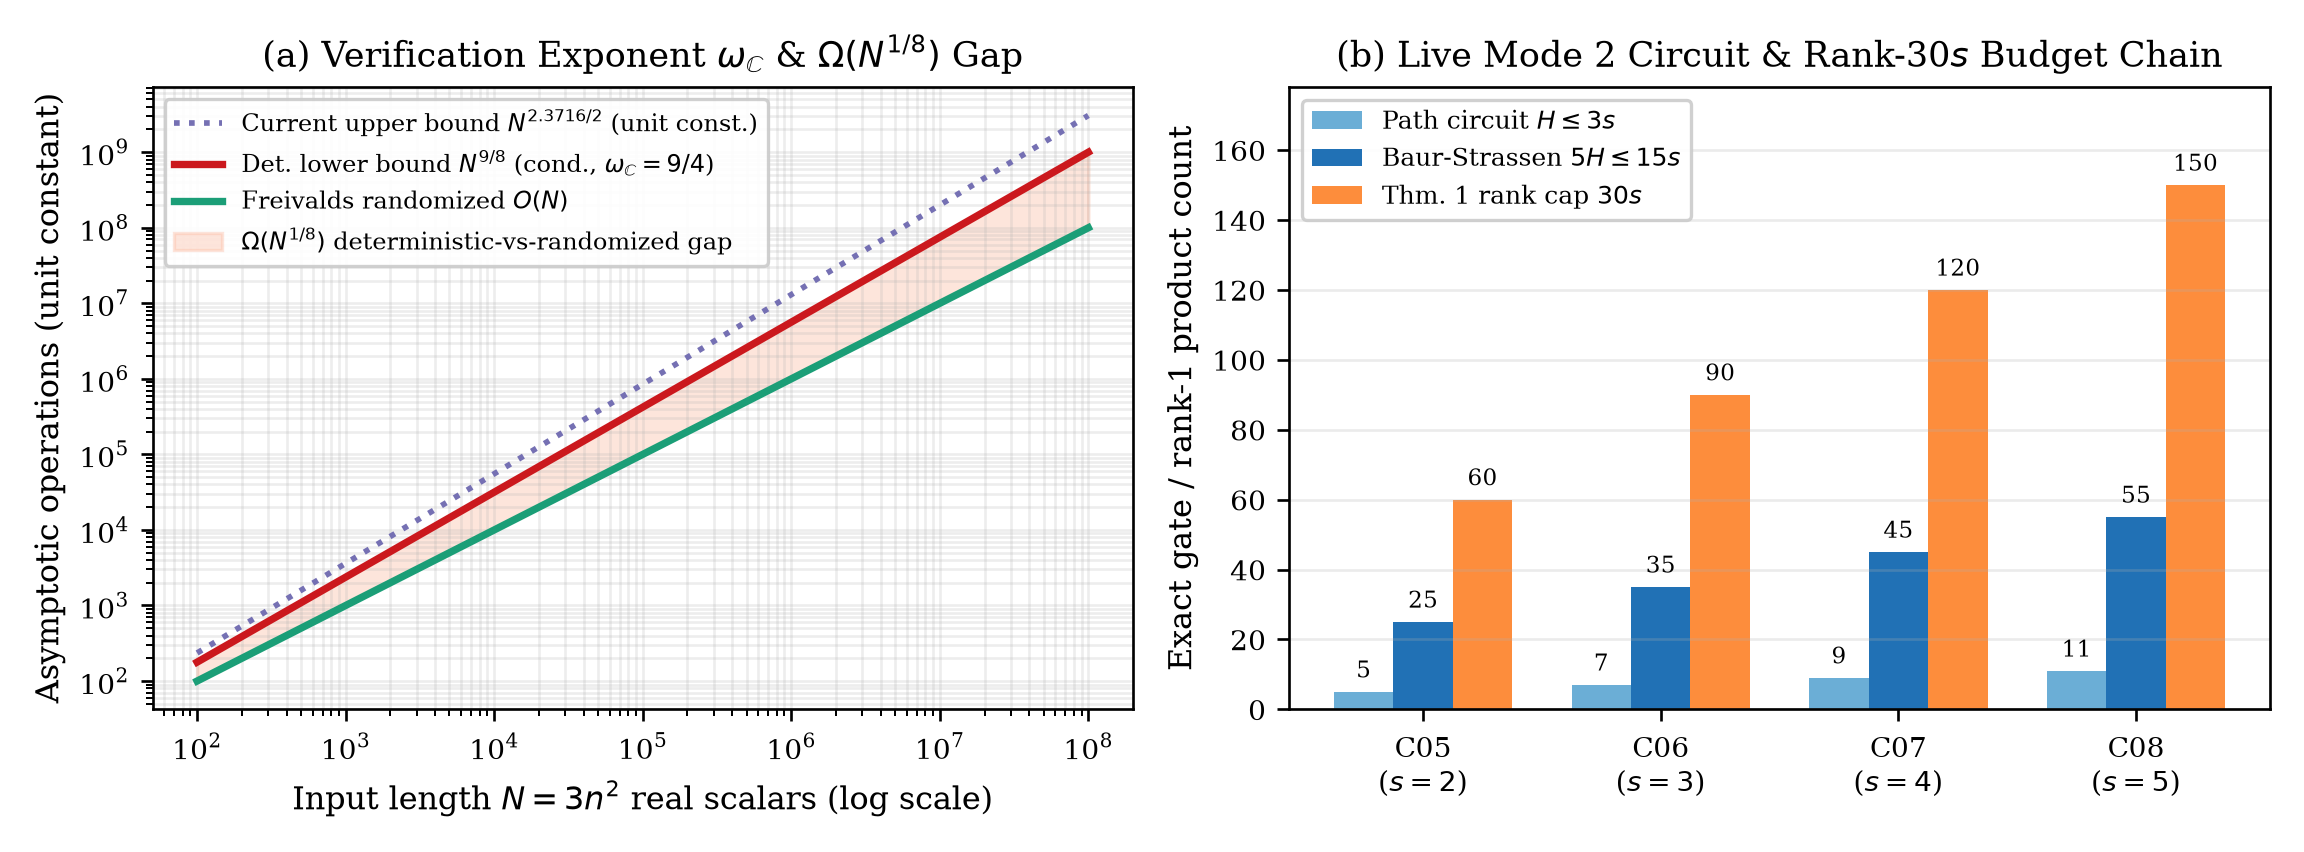
\includegraphics[width=0.84\textwidth]{figures/fig1_separation_and_rank_budget.png}
\caption{\textbf{Deterministic-vs.-Randomized Separation and $30s$ Budget.} (a)~Comparison of Freivalds' $O(N)$ test, conditional $\Omega(n^{9/4}) = \Omega(N^{9/8})$ lower bound~\cite{OpenAI2026NineFourths}, and current $n^{2.371552}$ upper bound~\cite{WilliamsXuXuZhou2024} (unit-constant scaling in $N=3n^2$). (b)~Live Mode~2 gate/rank budget chain $H\le 3s$, $5H\le 15s$, $30s$ (\texttt{C05}--\texttt{C08}).}
\label{fig:fig1}
\end{figure*}

\begin{figure*}[t]
\centering
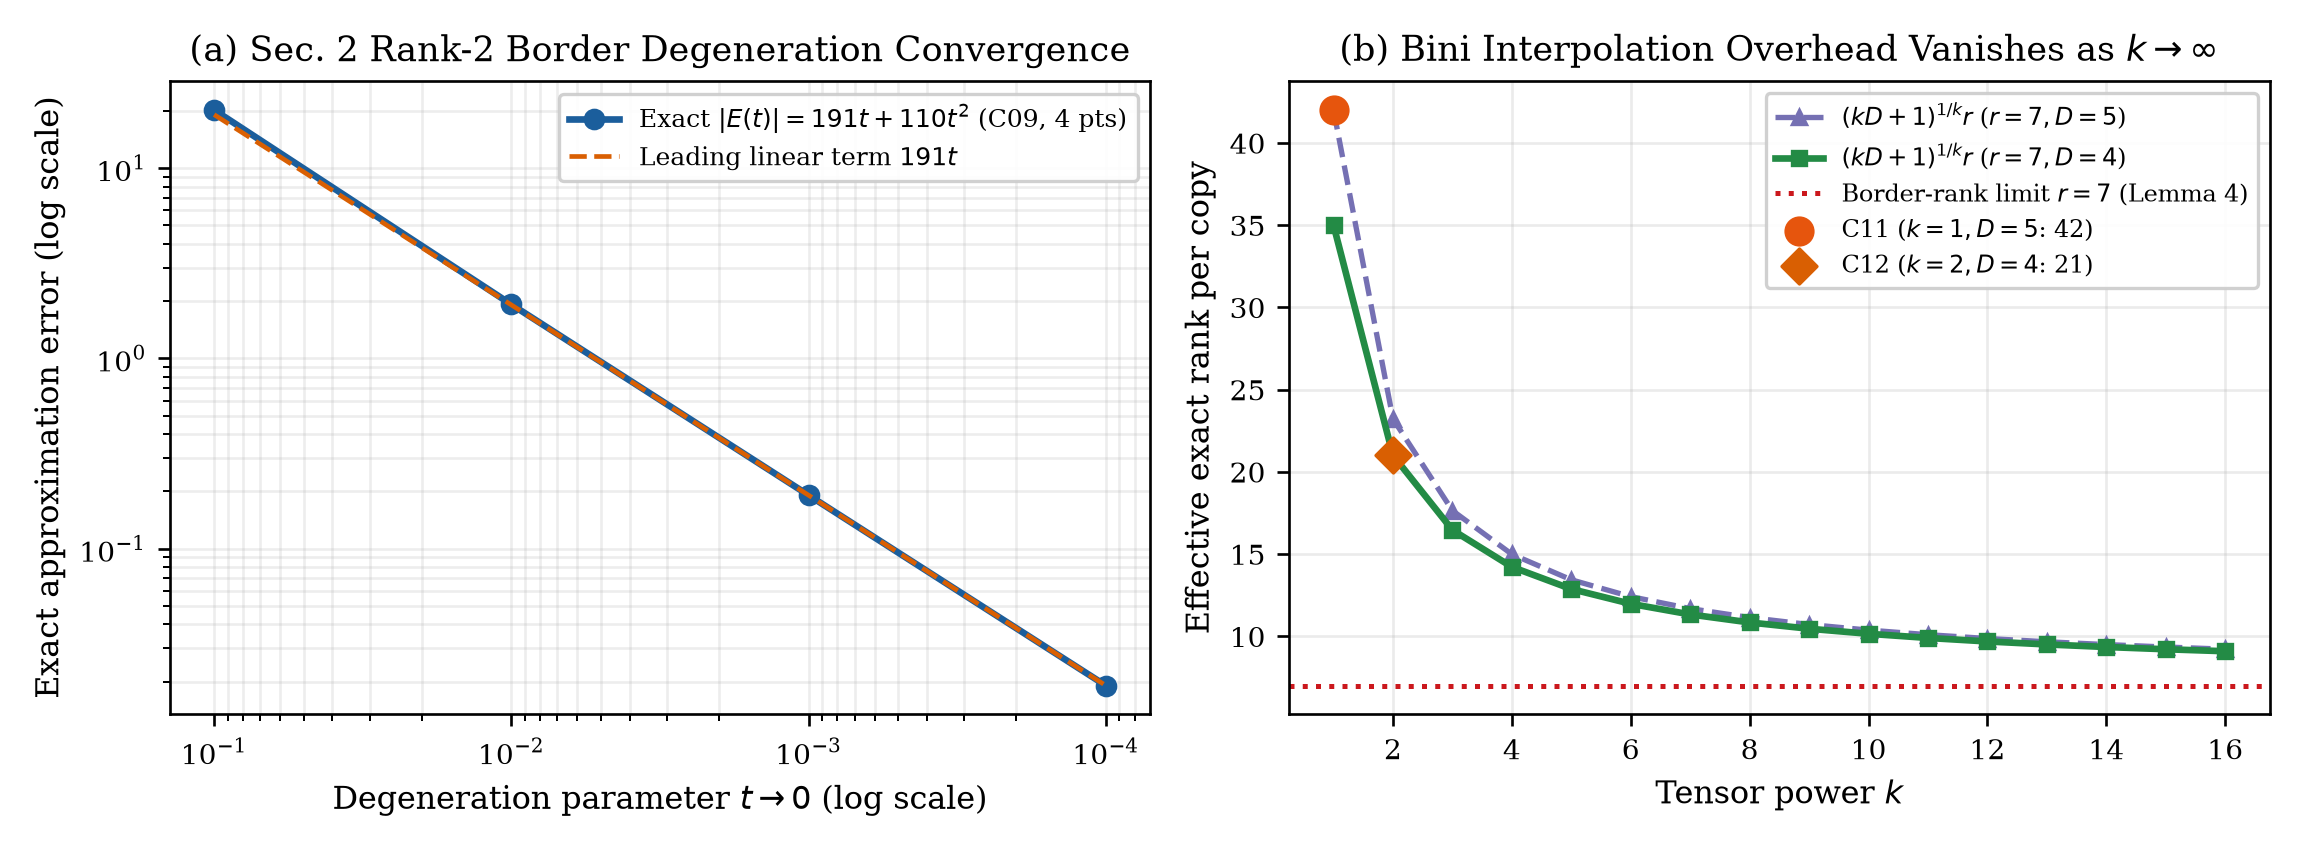
\includegraphics[width=0.84\textwidth]{figures/fig2_border_rank_and_bini.png}
\caption{\textbf{Border-Rank Degeneration and Bini Interpolation.} (a)~Exact $\mathbb{Q}$ convergence $|E(t)| = 191t + 110t^2$ of Section~2's rank-2 degeneration (\texttt{C09}). (b)~Vanishing of Bini's interpolation overhead $(kD+1)^{1/k} r \to r$ as $k\to\infty$ for $D=4$ and $D=5$, with live certified points \texttt{C11} ($D=5$) and \texttt{C12} ($D=4$).}
\label{fig:fig2}
\end{figure*}

\begin{figure*}[t]
\centering
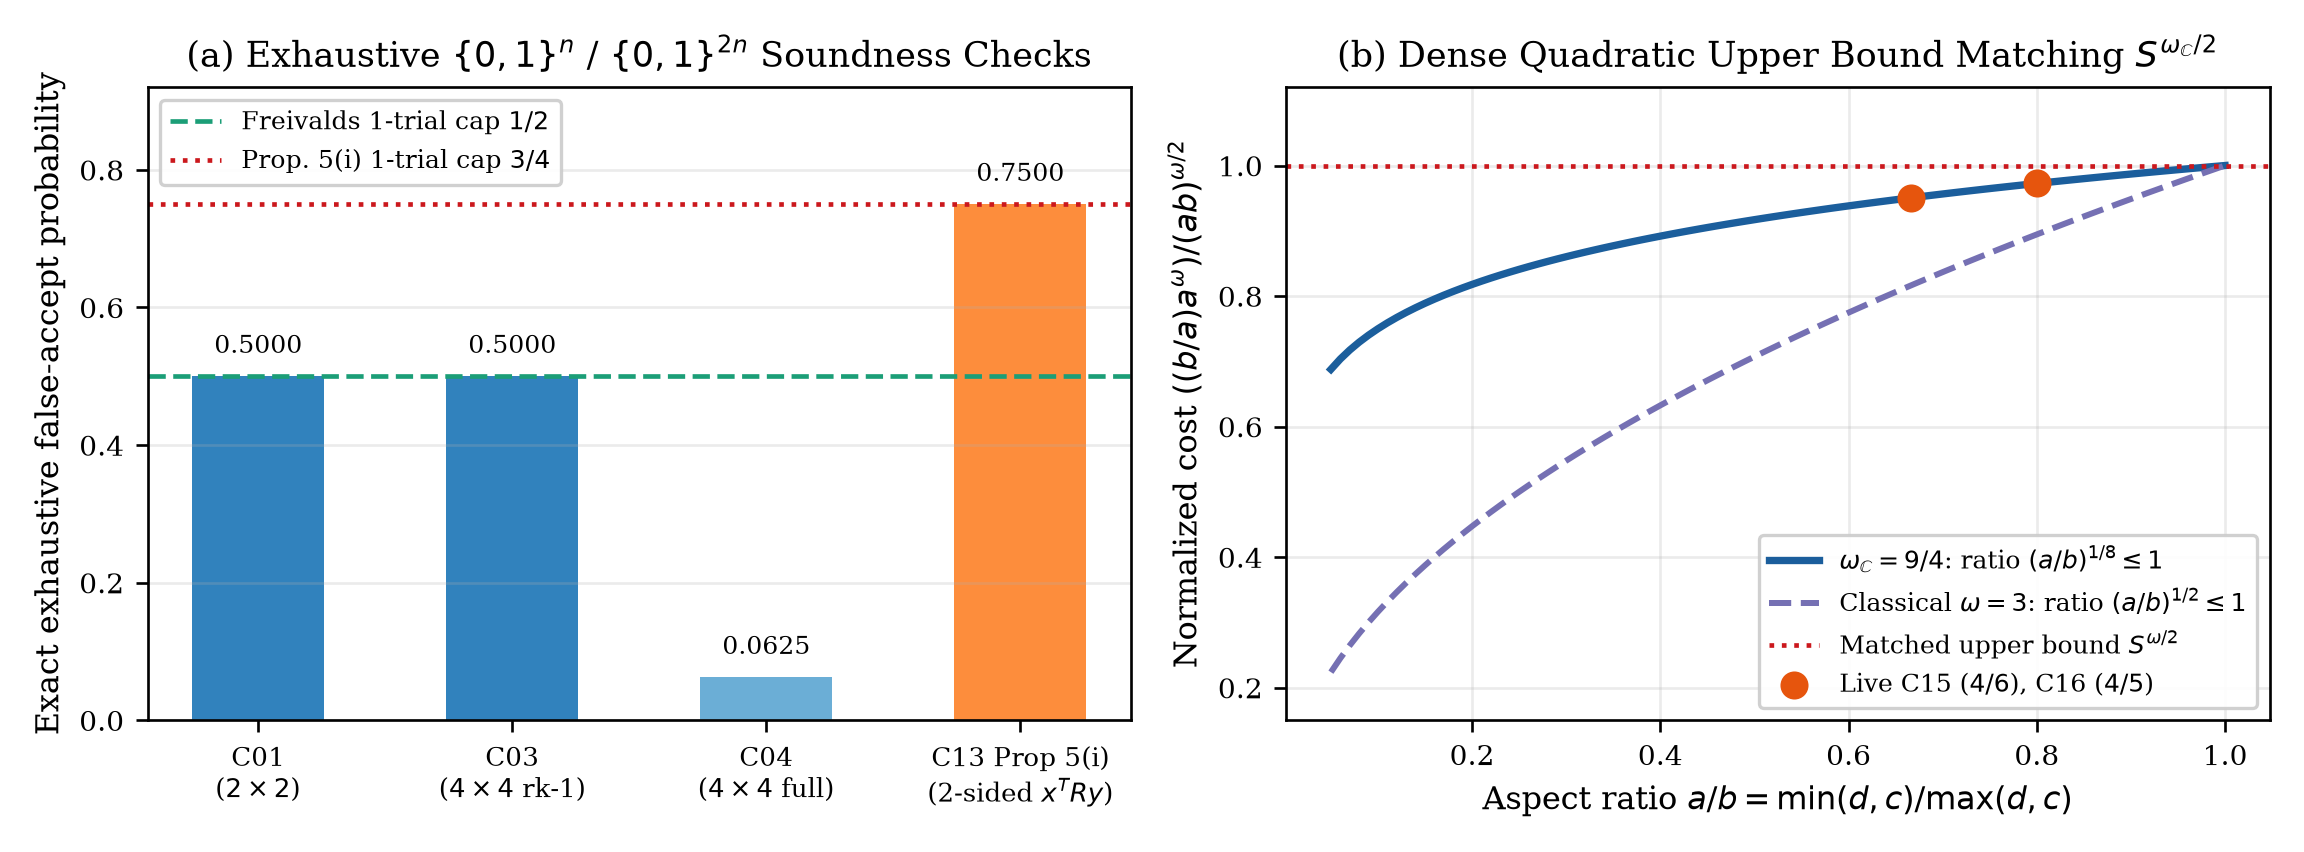
\includegraphics[width=0.84\textwidth]{figures/fig3_freivalds_and_pit_witnesses.png}
\caption{\textbf{Exhaustive Soundness and Dense-Quadratic Matching.} (a)~Exact exhaustive $\{0,1\}^n / \{0,1\}^{2n}$ false-accept rates across Modes~1 and~4a (\texttt{C01}, \texttt{C03}, \texttt{C04}, \texttt{C13}). (b)~Normalized dense quadratic cost $(a/b)^{\omega/2 - 1} \le 1$ confirming $(b/a)a^\omega \le (ab)^{\omega/2}$ for $\omega\in\{9/4, 3\}$ (\texttt{C15}, \texttt{C16}).}
\label{fig:fig3}
\end{figure*}

\paragraph{Worked Witness~1 (Dual-Ring Reciprocal and Cubic Gradient, \texttt{C06} \& \texttt{C08}).}
In \texttt{C06}, inverting $d = 3 + 2\alpha + 5\beta + 7\alpha\beta$ in $\mathbb{Q}[\alpha,\beta]/(\alpha^2,\beta^2)$ yields $d^{-1} = \tfrac{1}{3} - \tfrac{2}{9}\alpha - \tfrac{5}{9}\beta + (-\tfrac{7}{9} + \tfrac{2\cdot 2\cdot 5}{27})\alpha\beta = \tfrac{1}{3} - \tfrac{2}{9}\alpha - \tfrac{5}{9}\beta - \tfrac{1}{27}\alpha\beta$, which multiplies $d$ identically to $(1,0,0,0)$ while introducing only $1$ bilinear product ($d_1 d_2$). In \texttt{C08}, feeding $a=1+\alpha$, $b=2+\beta$, $c=3+\alpha$ into the cubic gradient circuit $(c-ab)^3$ gives $c-ab = 1-\alpha-\beta-\alpha\beta$, $(c-ab)^2 = 1-2\alpha-2\beta$, and $(c-ab)^3 = 1-3\alpha-3\beta+3\alpha\beta$, using $6$ bilinear products well inside Theorem~1's $30s = 150$ cap (Fig.~\ref{fig:fig1}b).

\paragraph{Worked Witness~2 (Bini Interpolation and Dense Quadratic Cancellation, \texttt{C12} \& \texttt{C16}).}
In \texttt{C12} ($M=1, D=4, r=7, k=2$), exact Lagrange interpolation over $\mathbb{Q}$ at $kD+1 = 9$ integer nodes recovers the degree-$kh = 6$ target coefficient $c_6 = 1764$ with exact rank cap $9\cdot 7^2 = 441$ (Fig.~\ref{fig:fig2}b). In \texttt{C16} ($d=5 > c=4, K=2$), choosing $R\in\mathbb{Q}^{5\times 4}$ with columns $(e_1, e_2, e_2, -e_1)$ gives $RJR^T = e_1 e_2^T - e_2 e_1^T + e_2 e_1^T - e_1 e_2^T = 0$ and $HJH = 0$ identically, while $5^8 \cdot 4^{10} = 409{,}600{,}000{,}000 \le 512{,}000{,}000{,}000 = 20^9$ verifies the $\omega_{\mathbb{C}}=9/4$ aspect-ratio bound over $\mathbb{Z}$.

\section{Reproducibility and Availability}
All source code, Lean~4 proofs, certificates, figure scripts, and SHA-256 manifest (\texttt{MANIFEST.sha256}) are archived at \nolinkurl{https://github.com/lluiseriksson/det-matrix-product-verification-certificates} under MIT (code/Lean/data) and CC-BY-4.0 (manuscript/figures) licenses. Reproduction requires three commands: \texttt{(cd lean \&\& lake build)}, \texttt{python -m} \nolinkurl{src.det_matmul_verif_verifier} \texttt{certificates}, and \texttt{pytest -q}.

\paragraph{AI Assistance Disclosure.}
Google Antigravity assisted with Lean~4 proof engineering, zero-float verifier implementation, test/figure automation, and LaTeX drafting. The author verified every mathematical derivation, Lean axiom audit, certificate check, and visual figure inspection, and takes full responsibility for all contents.

\bibliographystyle{plain}
\bibliography{references}
\end{document}
